
\documentclass[a4paper]{article}
\usepackage{mathtools}
\usepackage[utf8x]{inputenc}
\usepackage[pdftex]{graphicx}
\usepackage[usenames,dvipsnames,svgnames,table]{xcolor}
\usepackage{framed}
\usepackage[most]{tcolorbox}

\begin{document}
\title{Laboratorio 1}
\author{
        Tabacoff Mila Romana Cécile \\
        Magliona Marco \\
        Lecce Michela \\
        Della Monica Andrea}

\date{\today}
\maketitle


\begin{figure}[h]
\centering
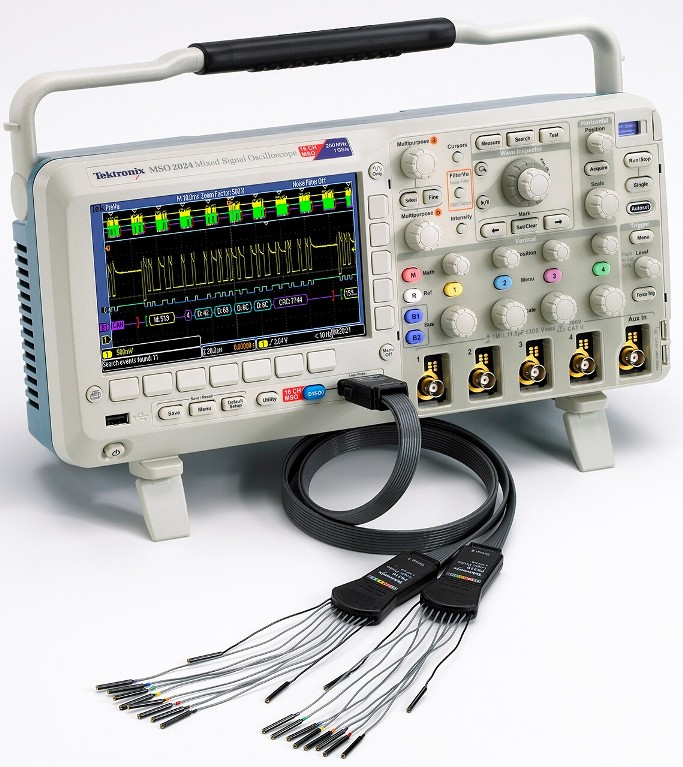
\includegraphics[scale=0.5]{dso.jpg}
\caption{un oscilloscopio}
\end{figure}


\begin{tcolorbox}[breakable,colback=cyan,colframe=cyan]
\section*{Misurazione di valore efficace e frequenza}
\end{tcolorbox}

\subsection{Misurazione del valore efficace}

\begin{itemize}
\item Lettura dell’ampiezza picco-picco {\(Vpp= V\)}
\item Formula impiegata per il calcolo dell’incertezza: Modello probabilistico \[\bar{n} = \tfrac{1}{m}\sum_{k=1}^m n_k \]
\[s^2 (n_k)= \tfrac{1}{m-1}\sum_{k=1}^m (n_k - \bar{n})^2 \] 
\[s^2 (\bar{n}) = \tfrac{s^2 (n_k)}{m}\]
\item Incertezza: \(\delta{}  Vpp= \)
\item Valore efficace e incertezza \(Veff \)
\end{itemize}

\subsection{Misurazione di frequenza}
\begin{itemize}
\item Formula incertezza:
\item \(T= s\pm s \)
\item \(f= Hz \pm Hz\)
\end{itemize}

\subsection{Verifica con multimetro}
\begin{itemize}
\item \(Veff= \pm V \)
\item \(f= Hz \pm Hz \)
\end{itemize}


\begin{tcolorbox}[breakable,colback=cyan,colframe=cyan]
\section*{Misurazione del tempo di salita}
\end{tcolorbox}


\subsection{ Misurazione 1}
\begin{itemize}
\item Il sistema in misura presenta un disadattamento d’impedenza il cui effetto `e quello di distorcere il fronte di salita del segnale. In queste condizioni il tempo di salita è \(ts1 = ns\)
\item Misurazione in condizioni di adattamento \(ts_2 = ns\) 
\item Tempo di salita introdotto dall’oscilloscopio a causa della sua banda passante \(tso=\tfrac{0.35}{B} = ns\)
\item \(ts= \sqrt{ts_2^2 -tso^2} = ns\)
\end{itemize}

\subsection{Misurazione 2}
\colorbox{ProcessBlue}{??? la faremo... forse}

\begin{enumerate}
\item Frequenza del polo ed effetto sulla misura del tempo di salita
  \begin{itemize}
    \item Capacità totale \(Ctot = pF\)
    \item Resistenza del generatore ”modificato” \(Rg= \)
    \item Frequenza polo \(fp = \tfrac{1}{2\pi \cdot Rg \cdot Ctot} = kHz \)
    \item Tempo di salita dovuto al polo \(tsp= 0.35/fp = ns\)
    \item Verifica sperimentale \(tsp_m = ns\)
    \end{itemize}

\item Per ridurre questo effetto sistematico utilizziamo la sonda compensata al posto del cavo coassiale
 \begin{itemize}
 \item  \(Cs= pf\)
 \item Frequenza polo \(fp' = kHz\)
 \item Nuovo tempo di salita atteso \(tsp'= ns\)
 \item \(tsp'\_m= ns\)
 \end{itemize}
\end{enumerate}



\begin{tcolorbox}[breakable,colback=cyan,colframe=cyan]
\section*{Aliasing}
\end{tcolorbox}


\subsection{Aliasing percettivo}
 \begin{enumerate}
  \item Abbiamo ridotto la velocità di scansione
  \item Velocità di scansione tale per cui la frequenza vale \(fco= 1 MHz\)
  \item Abbiamo impostato lo strumento per la visualizzazione a punti
  \item Modificato la frequenza del generatore
 \end{enumerate}

\subsection{Effetto dell’aliasing nel dominio del tempo}
 \begin{enumerate}
  \item Abbiamo impostato la frequenza del generatore di segnali a \(fg=100.1 kHz\)
  \item Abbiamo ridotto la frequenza di scansione fino ad avere una frequenza di campionamento di \(fco=100 kHz\) Abbiamo misurato la frequenza del segnale osservato \(fs= Hz\)
  \item Abbiamo portato la frequenza del generatore di segnali a \(fg=100khz\)
  \item Provato altre combinazioni di frequenza-segnale/frequenza-campionamento
\end{enumerate}


\begin{tcolorbox}[breakable,colback=cyan,colframe=cyan]
\section*{Rilevazione sincrona di segnali}
\end{tcolorbox}


\subsection{Operazioni preliminari}
 \begin{enumerate}
  \item circuito
  \item generatori regolati come
   \begin{itemize}
     \item GEN1
     \item GEN2
   \end{itemize}
  \item Segnale del canale 1 con oscilloscopio sincronizzato sul canale 1 e poi sul canale 2

\subsection{Misurazione}
  \item oscilloscopio sincronizzato sul canale 2 con l'opzione media
  \item Abbiamo modificato il segnale di disturbo e il numero di medie
  \item Effetto media quando l'oscilloscopio è sincronizzato sul canale 1
 \end{enumerate}

\noindent \LaTeX

\end{document}






